\chapter{Grundlagen}
% Der \gls{accesspoint} sendet die \gls{bssid} und die \gls{ssid}, damit Geräte, wie eine \gls{vm}, sich verbinden können. Algorithmen wie \gls{knn} und \gls{svm} können in einer \gls{api} implementiert werden, um die Datenverarbeitung zu optimieren.


% Quelle 1: Access Points Service Set Identifier (SSID) for Localization and Tracking -> masoud2022access
% Quelle 2: RSSI-Based Indoor Localization With the Internet of Things -> sadowski2018rssi
% Quelle 3: Survey on Indoor localization System and Recent Advances of WIFI Fingerprinting Technique -> basri2016survey

% Das ist eine Test Zitierung\myfootcite{TORRESSOSPEDRA20159263}{S. 23}.

\section{Indoor-Ortung via WiFi Fingerprints}

WiFi-Fingerprinting ist eine Technik die zur Lokalisierung in Innenräumen verwendet werden kann. Dabei werden an verschiedenen Positionen in einem Gebäude die Signalstärken der empfangenden WLAN-Router - die sogenannten Access Points - gemessen und in einer Datenbank gespeichert. Dadurch dass an verschiedenen Positionen verschiedene Access Points unterschiedlich stark empfangen werden, entsteht eine Art Fingerabdruck dieser Position, welcher verwendet werden kann um die Position eines Geräts anhand der empfangenen Access Points und deren Signalstärke zu bestimmen.

Das Prinzip der WiFi-Fingerprinting-basierten Ortung kann in eine Offline- und eine Online-Phase unterteilt werden. In der Offline-Phase werden die Fingerprints aufgezeichnet und mit den dazugehörigen Positionen gespeichert. In der Online-Phase wird die aktuelle Position eines Geräts bestimmt, indem dieses ebenfalls einen WiFi-Fingerprint aufzeichnet und diesen mit den bekannten Fingerprints in der Datenbank abgleicht. Die Position des Geräts wird anschließend anhand des am besten passenden Fingerprints bestimmt. 

Neben der Indoor-Ortung mittels WiFi-Fingerprinting können auch andere Technologien wie Bluetooth, Ultra-wideband, RFID und Zigbee verwendet werden, wobei jede Technik seine Vor- und Nachteile mit sich bringt. Die Vorteile des WiFi-Fingerprinting sind, dass diese in vielen Fällen verwendet werden kann ohne zusätzliche Hardware zu installieren, da die meisten Gebäude bereits über eine WLAN-Infrastruktur verfügen. Zudem ist die Reichweite von WLAN-Signalen größer als die von Bluetooth oder RFID, wodurch insgesamt weniger Hardware benötigt wird. Der Nachteil dieser Technik ist jedoch der zeitliche Aufwand beim Erstellen der Fingerprints während der Offline-Phase\myfootcite{Shang2022WiFiFingerprinting}{S. 726 ff.}.

\section{Technische Grundlagen}

Ein WiFi-Fingerprint kann definiert werden als eine Liste der empfangenen Access Points, wobei in jedem Eintrag die MAC-Adresse und die Signalstärke steht.\myfootcite{Shang2022WiFiFingerprinting}{S. 729} In dieser Arbeit wurden diese Einträge um die Klarnamen der Netzwerke - die so genannte SSID - erweitert.

\subsection{BSSID}

Der Basic Service Set Identifier (BSSID) ist die eindeutige Kennung eines Access Points und entspricht der MAC-Adresse des Access Points. Diese Adresse ist unveränderlich und kann dazu verwendet werden  einen Access Point eindeutig zu identifizieren.\myfootcite{Amirisoori2017}{S. 27}

\subsection{SSID}

Der Service Set Identifier (SSID) ist ein eindeutiger Bezeichner, der ein drahtloses Netzwerk kennzeichnet und aus einer alphanumerische Zeichenfolgen - wie zum Beispiel \textit{eduroam} oder \textit{FRITZ!Box 7590 XY} - besteht. Im Gegensatz zur BSSID kann die SSID frei gewählt werden, wodurch mehrere Access Points die selbe SSID haben können.\myfootcite{masoud2022access}{S. 5460} % (Quelle 1, Kapitel 1, Seite 5460).

\subsection{RSSI} \label{rssi}

Der Received Signal Strength Indicator (RSSI) ist ein relativer Indikator für die Empfangsstärke eines kabellosen Kommunikationssystems nach IEEE 802.11 Standard und gibt die Qualität eines empfangen Signals auf einer Skale von -100 bis 0 in der Einheit dBm an. Je größer der Wert ist, also je näher dieser an 0 ist, desto besser ist das Signal.\mycitefoot{iotmeshRSSIReceived}

\section{Zusammenhang zwischen Signalstärke und Distanz} \label{pfadverlustmodell}

Da für Indoor-Ortung mittels WiFi-Fingerprints die RSSI-Werte der Access Points verwendet werden, ist es hilfreich den Zusammenhang zwischen der Signalstärke un der Entfernung zu verstehen. Die RSSI-Werte sind abhängig von der Entfernung zwischen dem Sender und dem Empfänger und nehmen mit zunehmender Distanz ab. Der Zusammenhang zwischen dem RSSI-Wert und der Entfernung kann durch das Pfadverlustmodell (siehe Gleichung \ref{eq:rssi}) beschrieben werden.

\begin{equation}
    RSSI = -10 * n * \log_{10}(d) + C
    \label{eq:rssi}
\end{equation}

Dabei ist \(n\) der Pfadverlustexponent, der je nach Umgebung variiert, \(d\) die Distanz zwischen Sender und Empfänger und \(C\) eine Konstante, die die Systemverluste berücksichtigt.\myfootcite{sadowski2018rssi}{S. 30153}

In dem Paper \textit{RSSI-Based Indoor Localization With the Internet of Things} wurden die Parameter des Pfadverlustmodells experimentell in einer Umgebung untersucht, welche mit der in dieser Arbeit verwendeten vergleichbar ist.\mycitefoot{sadowski2018rssi} Die Experimente wurden in einem Forschungslabor (10,8 m x 7,3 m) - welches mit mehreren WiFi- und Bluetooth-Geräten und Computern ausgestattet ist - durchgeführt. In dieser Umgebung ergaben die Untersuchungen einen Pfadverlustexponenten von \(n = 2.013\) und eine Konstante von \(C = -49.99\) dBm.\myfootcite{sadowski2018rssi}{S. 30157}

Das Pfadverlustmodell mit den Ergebnissen aus der erwähnten Studie ist in Abbildung \ref{fig:plot_rssi_distance} dargestellt und dient als Grundlage für die in Kapitel \ref{datenaufbereitung} untersuchten Datenaufbereitungsschritte.

\begin{figure}[H]
    \centering
    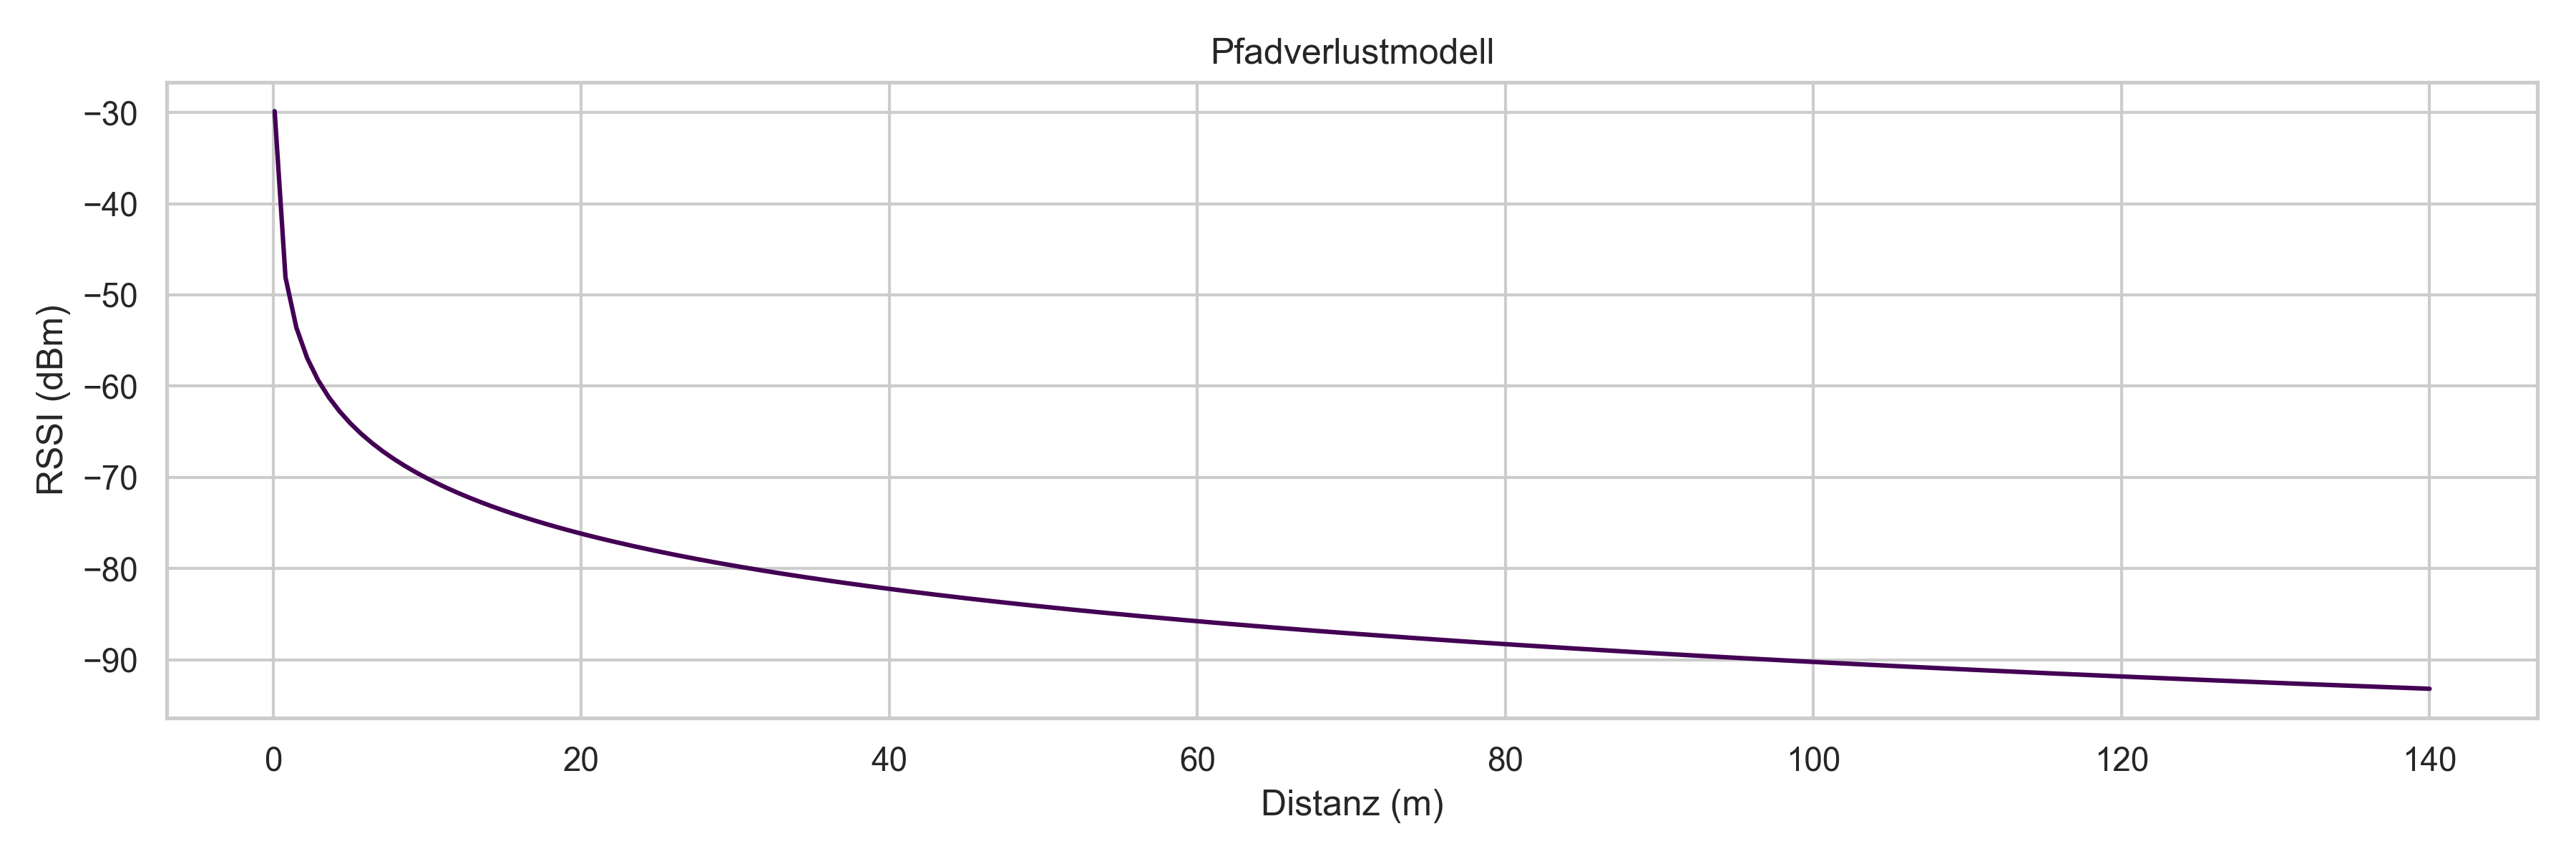
\includegraphics[width=0.8\textwidth]{images/plot_rssi_distance.png}
    \caption{Exemplarischer Zusammenhang zwischen RSSI-Werten und der Entfernung nach dem Pfadverlustmodell}
    \label{fig:plot_rssi_distance}
\end{figure}